\documentclass[a4paper]{article}
\usepackage[utf8]{inputenc}
\usepackage[russian,english]{babel}
\usepackage[T2A]{fontenc}
\usepackage[left=10mm, top=20mm, right=18mm, bottom=15mm, footskip=10mm]{geometry}
\usepackage{indentfirst}
\usepackage{amsmath,amssymb}
\usepackage[italicdiff]{physics}
\usepackage{graphicx}
\graphicspath{{images/}}
\DeclareGraphicsExtensions{.pdf,.png,.jpg}
\usepackage{wrapfig}
\usepackage{float}
\usepackage{subcaption}
\usepackage{enumitem}
\usepackage{caption}
\usepackage{array}
\captionsetup[figure]{name=Рисунок}
\captionsetup[table]{name=Таблица}

\title{\underline{Отчет о выполненой лабораторной работе 4.1.1-4.1.2}}
\author{Воронин Денис, Б04-407}

\begin{document}

\maketitle

\begin{center}
\textbf{\Large Геометрическая оптика}
\end{center}

\textbf{Цель работы:} изучить методы определения фокусных расстояний
линз и сложных оптических систем; определить характеристики оптической системы, составленной из тонких линз; изучить недостатки
реальных линз сферическую и хроматическую аберрации, изучить модели зрительных труб (астрономической
трубы Кеплера и земной трубы Галилея) и микроскопа, определить
их увеличения.

\textbf{В работе используются:} оптическаяскамьяснаборомрейтеров, положительные и отрицательные линзы, экран, осветитель с ирисовой
диафрагмой, зрительная труба, светофильтры, кольцевые диафрагмы, линейка.

\section{Аннотация}

После выполнения работы должны получить: фокусные расстояния линз с помощью подзорной трубы, измеренные фокусные расстояния линз по формуле тонкой линзы и
методом Бесселя, собрать и изучить подзорные трубы Кеплера и Галилея, собрать и изучить модель микроскопа, изучить составную оптическую систему.

\section{Теоретический сведения}

\subsection*{Определение фокусного расстояния тонкой собирающей линзы
и сложных оптических систем по методу Аббе}
Измерение фокусного расстояния по методу Аббе основано на определении поперечного увеличения для нескольких (не менее двух) различных положений предмета

\begin{figure}[!hb]
	\centering
	
\includegraphics[width=0.8\linewidth]{p1.png}
	\caption{ Измерение фокусного расстояния оптической
системы по методу Аббе}
	\label{pic_1}
\end{figure}

Фокусное расстояние системы вычисляется с помощью выражения:

\begin{equation}
f = \frac{\Delta x}{\Delta (y / y')} = -\frac{\Delta x'}{\Delta (y' / y)}.
\label{eq:focal_length_ratio}
\end{equation}

Здесь $\Delta x = x_2 - x_1$ — смещение предмета, $\Delta x' = x_2' - x_1'$ — соответствующее ему перемещение изображения, $\Delta(y'/y) = y_2'/y_2 - y_1'/y_1$ — приращение поперечного увеличения, а $\Delta(y/y')$ — приращение величины, обратной поперечному увеличению.

\subsection*{Определение фокусного расстояния собирающих линз и сложных
оптических систем по методу Бесселя}

Схема метода Бесселя для случая, когда $n = n'$ и $f' = -f$, представлена на рис.~2. Она основана на том, что при заданном расстоянии $L$ между предметом и экраном уравнение
\begin{equation}
-\frac{1}{s} + \frac{1}{L - \delta + s} = \frac{1}{f}
\label{eq:bessel_method}
\end{equation}
представляет собой квадратное уравнение относительно расстояния $s$ от главной плоскости пространства предметов до предмета ($s < 0$).

\begin{figure}[!hb]
	\centering
	
\includegraphics[width=0.5\linewidth]{p2.png}
	\caption{ Измерение фокусного расстояния оптической
системы по методу Бесселя}
	\label{pic_1}
\end{figure}

\begin{equation}
f = \frac{L^2 - \ell^2}{4L}.
\label{eq:bessel_focal_length}
\end{equation}

Для определения фокусного расстояния $f$ достаточно, таким образом, измерить расстояние $L$ между предметом и экраном и расстояние $\ell$ между двумя положениями системы, при которых на экране видны чёткие изображения. Допускаемая при этом относительная погрешность результата измерений (без учёта случайных ошибок) даже для толстых линз и некоторых сложных оптических систем может быть мала.

\subsection*{Определение фокусного расстояния тонкой собирающей линзы}

Если собирающую линзу можно считать тонкой, т.е. принять, что
главные плоскости линзы совпадают, то её фокусное расстояние может быть измерено, например, следующими способами (в дополнение к изложенным выше).

\textbf{Способ 1.} Воспользуемся формулой тонкой линзы~\eqref{eq:thin_lens}:
\begin{equation}
-\frac{1}{a} + \frac{1}{a'} = \frac{1}{f}.
\label{eq:thin_lens_sign_convention}
\end{equation}
Здесь $a$ и $a'$ — расстояния предмета и его изображения от плоскости линзы, причём $a < 0$, $a' > 0$, если предмет находится слева, а его изображение — справа от линзы; фокусное расстояние $f > 0$.

\textbf{Способ 2}

Фокусное расстояние тонкой собирающей линзы можно
определить с помощью зрительной трубы, настроенной на бесконечность, то есть на параллельный пучок лучей. Разместив между предметом и зрительной трубой положительную линзу и перемещая её вдоль
оси системы, можно найти резкое изображение предмета в окуляре зрительной трубы. При этом расстояние от середины линзы до предмета
равно фокусному расстоянию тонкой линзы. Для толстой линзы зрительная труба позволяет определить только положение главного фокуса.

\subsection*{Определение фокусного расстояния тонкой рассеивающей линзы}
\newpage
\textbf{Способ 1.} Определение фокусного расстояния рассеивающей линзы затруднено тем, что изображение предмета получается мнимым (при действительном источнике) и поэтому не может быть получено на экране. Эту трудность легко обойти с помощью вспомогательной собирающей линзы.

\begin{figure}[!hb]
	\centering
	
\includegraphics[width=0.5\linewidth]{p3.png}
	\caption{ Измерение фокусного расстояния
рассеивающей линзы}
	\label{pic_1}
\end{figure}

\textbf{Способ 2.} Если расстояние $a$ на рис.~3 совпадает с модулем фокусного расстояния рассеивающей линзы, то изображение $S_2$ перемещается в бесконечность, то есть лучи выходят из линзы параллельным пучком.

Параллельность пучка можно установить с помощью зрительной трубы, настроенной на бесконечность. Зная расстояние от первой линзы до точки $S_1$ и расстояние между линзами, нетрудно определить фокусное расстояние тонкой рассеивающей линзы. Для толстой отрицательной линзы этот метод позволяет определить только положение главного фокуса.

\subsection{Определение положения главных и фокальных плоскостей сложной
оптической системы}

Для нахождения главных плоскостей системы недостаточно знать фокусное расстояние; нужно определить ещё положения главных фокусов. Это можно сделать при помощи зрительной трубы, настроенной на бесконечность. Отложив от главных фокусов отрезки, равные фокусному расстоянию, можно найти положения главных плоскостей системы. При этом необходимо учитывать возможность различного взаимного расположения кардинальных точек (плоскостей) сложной системы.

\section{Ход работы}

\subsection{Подготовка к работе}

Сделали подготовку согласно описанию.

\subsection{Определение фокусных расстояний линз с помощью подзорной трубы}

Определили фокусные расстояния для собирающих линз:\par

1. Линза 5.6: 4,6 см.\par
2. Линза 5.3: 20,0 см.\par
3. Линза 5.2: 15,5 см.\par
4. Линза 5.1: 8,0 см.\par
5. Линза 5.4: 30,0 см.\par

Измерим фокусное расстояние рассеивающей линзы:\par

\begin{enumerate}
    \item[\textbf{а)}] Я разместил на скамье перед источником~И положительную линзу~Л$_1$ с наибольшим из имеющихся фокусным расстоянием~$f_1$. Я получил на экране~Э за линзой чёткое изображение предмета (лучше, если изображение будет немного \textit{уменьшенным}). Я учёл, что расстояние от предмета до действительного изображения не может быть меньше, чем~$4f_1$!
    
    \item[\textbf{б)}] Я измерил расстояние от линзы до экрана~$b_1 = 28,5$ см. Я убедился, что $b_1$ больше, чем предполагаемое $|f_p|$ отрицательной линзы (в противном случае я подобрал другое расположение линзы и экрана или использовал более длиннофокусную линзу);
\end{enumerate}

\newpage

\begin{figure}[!hb]
	\centering
	
\includegraphics[width=0.5\linewidth]{p4.png}
	\label{pic_1}
\end{figure}

\begin{figure}[!hb]
	\centering
	
\includegraphics[width=0.5\linewidth]{p5.png}
	\label{pic_1}
\end{figure}

\begin{enumerate}
    \item[\textbf{в)}] Я поместил исследуемую отрицательную линзу~Л$_\text{р}$ между~Л$_1$ и экраном (изображение~$y_1$ стало для неё \textit{мнимым предметом});
    
    \item[\textbf{г)}] Я убрал экран и за отрицательной линзой разместил подзорную трубу~П; перемещая отрицательную линзу по скамье (положительная~--- неподвижна!), я получил сфокусированное изображение предмета в подзорную трубу. Для повышения чёткости картины я использовал диафрагму~Д~$\varnothing 5$~мм.
    
    \item[\textbf{д)}] Я измерил расстояние~$l = 19,5$ см между линзами и определил фокусное расстояние рассеивающей линзы:
    \begin{equation}
        f_\text{р} = -(b_1 - l) = -9 \text{см}.
    \end{equation}
\end{enumerate}

\newpage
\subsection{Измерение фокусных расстояний линз по формуле тонкой линзы и
методом Бесселя}

\begin{figure}[!hb]
	\centering
	
\includegraphics[width=0.5\linewidth]{p5.png}
	\label{pic_1}
\end{figure}

\begin{enumerate}
    \item Я выбрал одну из положительных линз с известным (приближённо) значением фокусного расстояния~$f$. Я поместил экран на некотором расстоянии~$L > L_{\min} = 4f$ от предмета. Я измерил~$L = 71$ см.
    
    \item Я поместил исследуемую линзу между источником и экраном и нашёл два её положения, при которых на экране возникают чёткие действительные изображения~--- в одном случае увеличенное, а в другом уменьшенное. Я измерил соответствующие расстояния~$a_1 = 21,7$ см и~$a_2 = 50,6$ см от источника до линзы.
\end{enumerate}

\begin{enumerate}
    \setcounter{enumi}{2}
    
    \item Я вычислил фокусные расстояния линз:
    
    \begin{enumerate}
        \item[\textbf{а)}] По формуле тонкой линзы:
        \begin{equation}
            \frac{1}{f} = \frac{1}{a} + \frac{1}{L - a}.
        \end{equation}
    \end{enumerate}
\end{enumerate}

\[f = \frac{a(L-a)}{L} = 15,06 \pm 0,09 \text{см} \]

\newpage

\subsection{Сборка и изучение подзорных труб Кеплера и Галилея}

\begin{figure}[!hb]
	\centering
	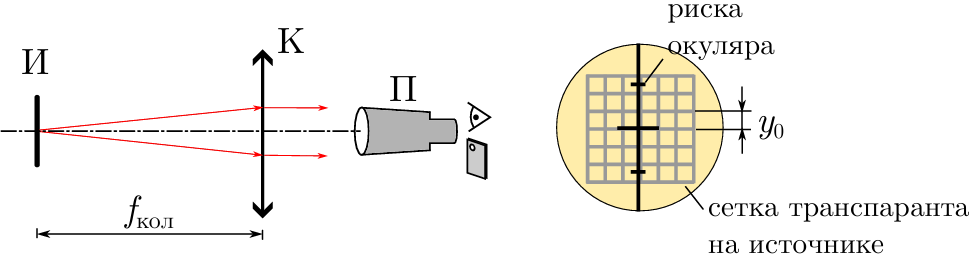
\includegraphics[width=0.8\linewidth]{p7.png}
	\label{pic_1}
\end{figure}

\begin{figure}[!hb]
	\centering
	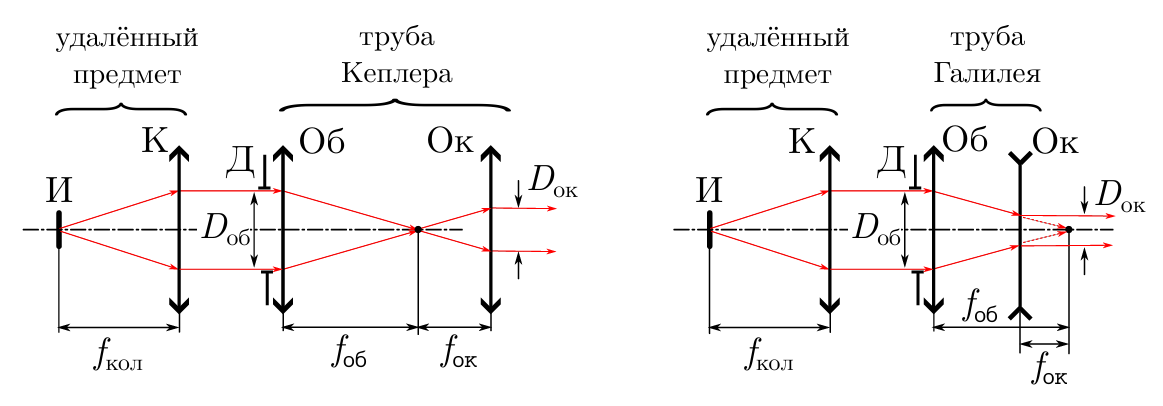
\includegraphics[width=0.8\linewidth]{p8.png}
	\label{pic_1}
\end{figure}

\begin{enumerate}
    \item Я выбрал из имеющегося набора линз три: две линзы для \textit{объектива}~$f_\text{об} = 5.4$ и \textit{окуляра}~$f_\text{ок} = 5.5$, чтобы расчётное угловое увеличение телескопа было равно $|\gamma| = |f_\text{об}/f_\text{ок}| \sim 2 \div 4$, и одну из собирающих линз для использования в качестве \textit{коллиматора}~$f_\text{кол} = 5.2$ (устройства для получения параллельного пучка света). Для коллиматора я решил использовать одну из наиболее длиннофокусных линз.
    
    \item С помощью вспомогательной подзорной трубы~П я установил коллиматорную линзу перед источником так, чтобы транспарант оказался строго в фокусе линзы (как при измерении фокусных расстояний в упражнении~I). Таким образом, я создал расположенный на бесконечности предмет с угловым размером $\alpha_0 = y_0/f_\text{кол}$, который я затем рассматривал с помощью модели телескопа.
\end{enumerate}

\begin{enumerate}
    \setcounter{enumi}{2}
    
    \item Я сфотографировал на камеру смартфона картину, наблюдаемую в окуляр вспомогательной подзорной трубы~П.
Угловой размер: $\alpha_{1} = 1/9$
\end{enumerate}

\begin{figure}[!hb]
	\centering
	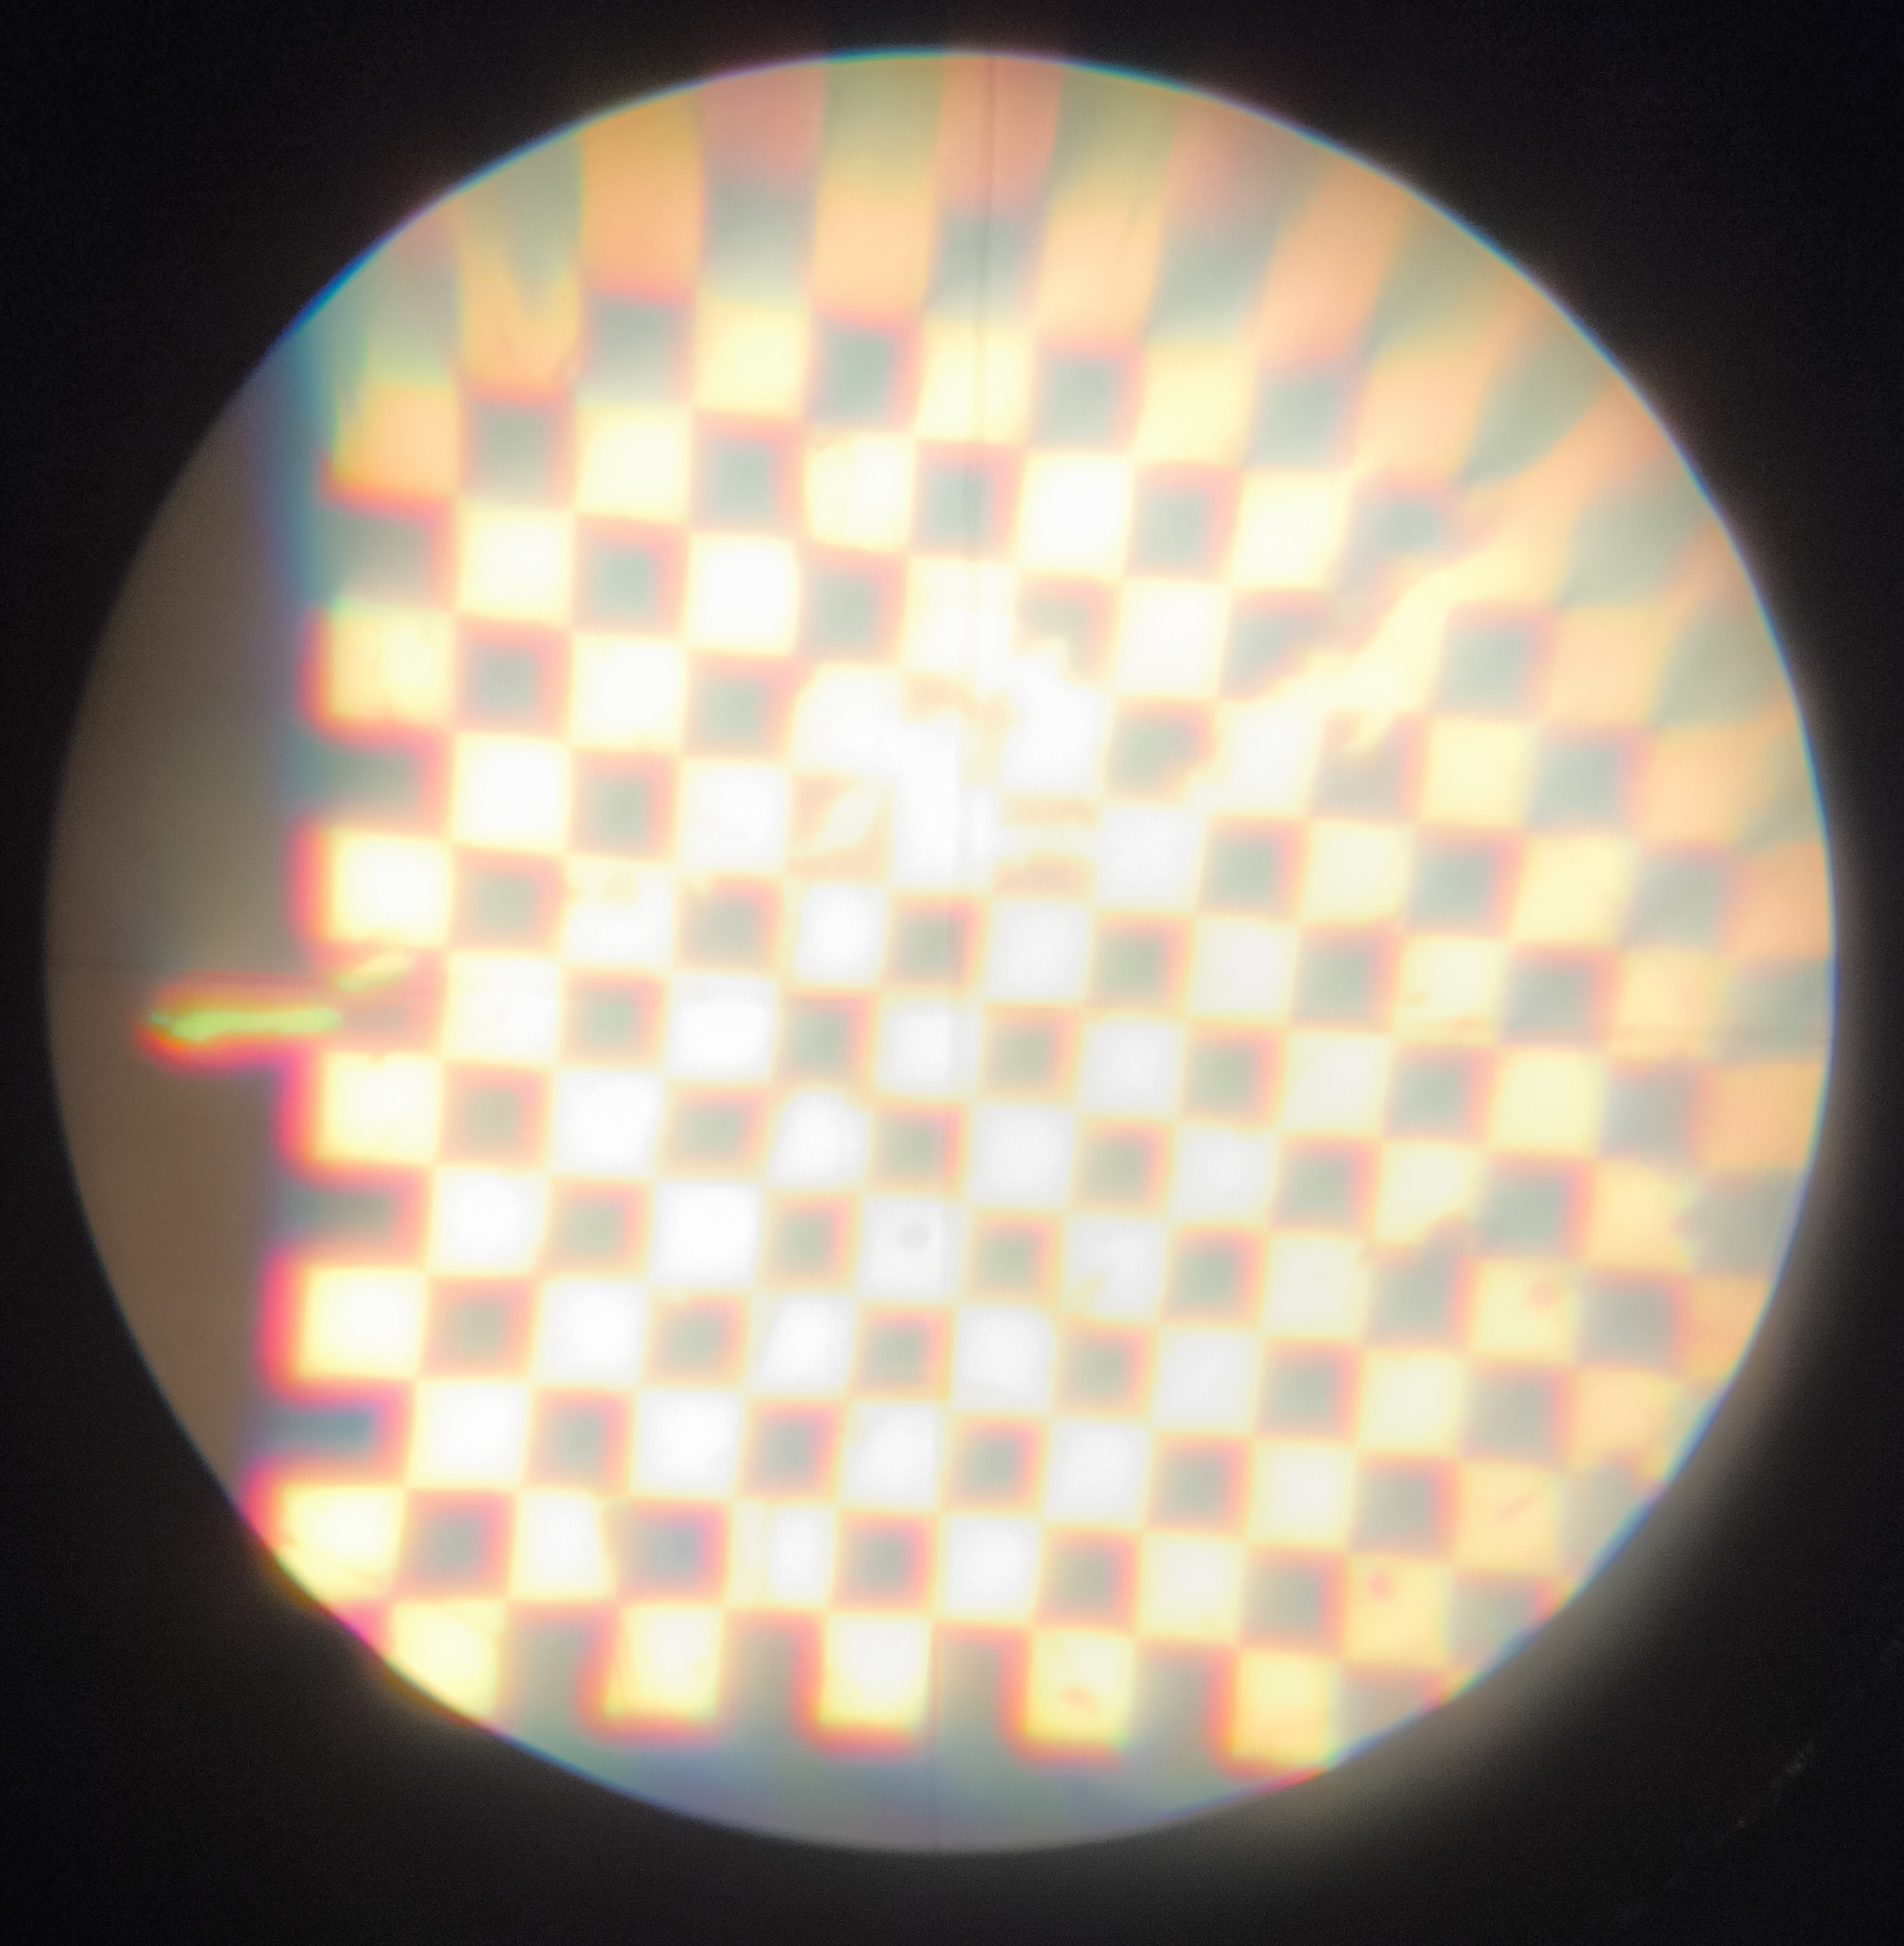
\includegraphics[width=0.4\linewidth]{f2.jpg}
	\label{pic_1}
\end{figure}

\newpage

\begin{enumerate}
    \setcounter{enumi}{3}
    
    \item Я собрал на скамье модель телескопа Кеплера (или Галилея). Собирающую линзу с наибольшим (по модулю) фокусным расстоянием~--- объектив телескопа~--- я расположил сразу за коллиматором. Вторую линзу (собирающую или рассеивающую)~--- окуляр телескопа~--- я установил на расстоянии $f_\text{об} + f_\text{ок}$ от объектива (для трубы Галилея $f_\text{ок} < 0$).
\end{enumerate}

\begin{enumerate}
    \setcounter{enumi}{4}
    
    \item При непосредственном наблюдении глазом через окуляр <<телескопа>> я наблюдал увеличенное изображение сетки на поверхности источника. Чёткость изображения я существенно повысил, когда разместил на коллиматоре или объективе дополнительную диафрагму~$\varnothing 5$~мм.
    
    \item Для нахождения углового увеличения собранного телескопа я измерил новый видимый размер~$\alpha_{2} = 1/2.5$ изображения ячейки сетки осветителя.
    
    Для этого я вновь установил вспомогательную подзорную трубу на скамью непосредственно за окуляром моей модели телескопа и повторил измерение углового размера ячейки аналогично п.~3 (я сопоставил размеры элементов на фотографиях в графическом редакторе, либо определил число ячеек сетки, укладывающихся на размере окулярной риски). Я рассчитал увеличение $\gamma_\text{эксп} = \alpha/\alpha_0 = 3,6$ и сравнил его с теоретическим $\gamma_\text{теор} = |f_\text{об}/f_\text{ок}| = 3,33$. Я проанализировал, в чём могут быть причины расхождения теории и измерений.
\end{enumerate}

\begin{figure}[!hb]
	\centering
	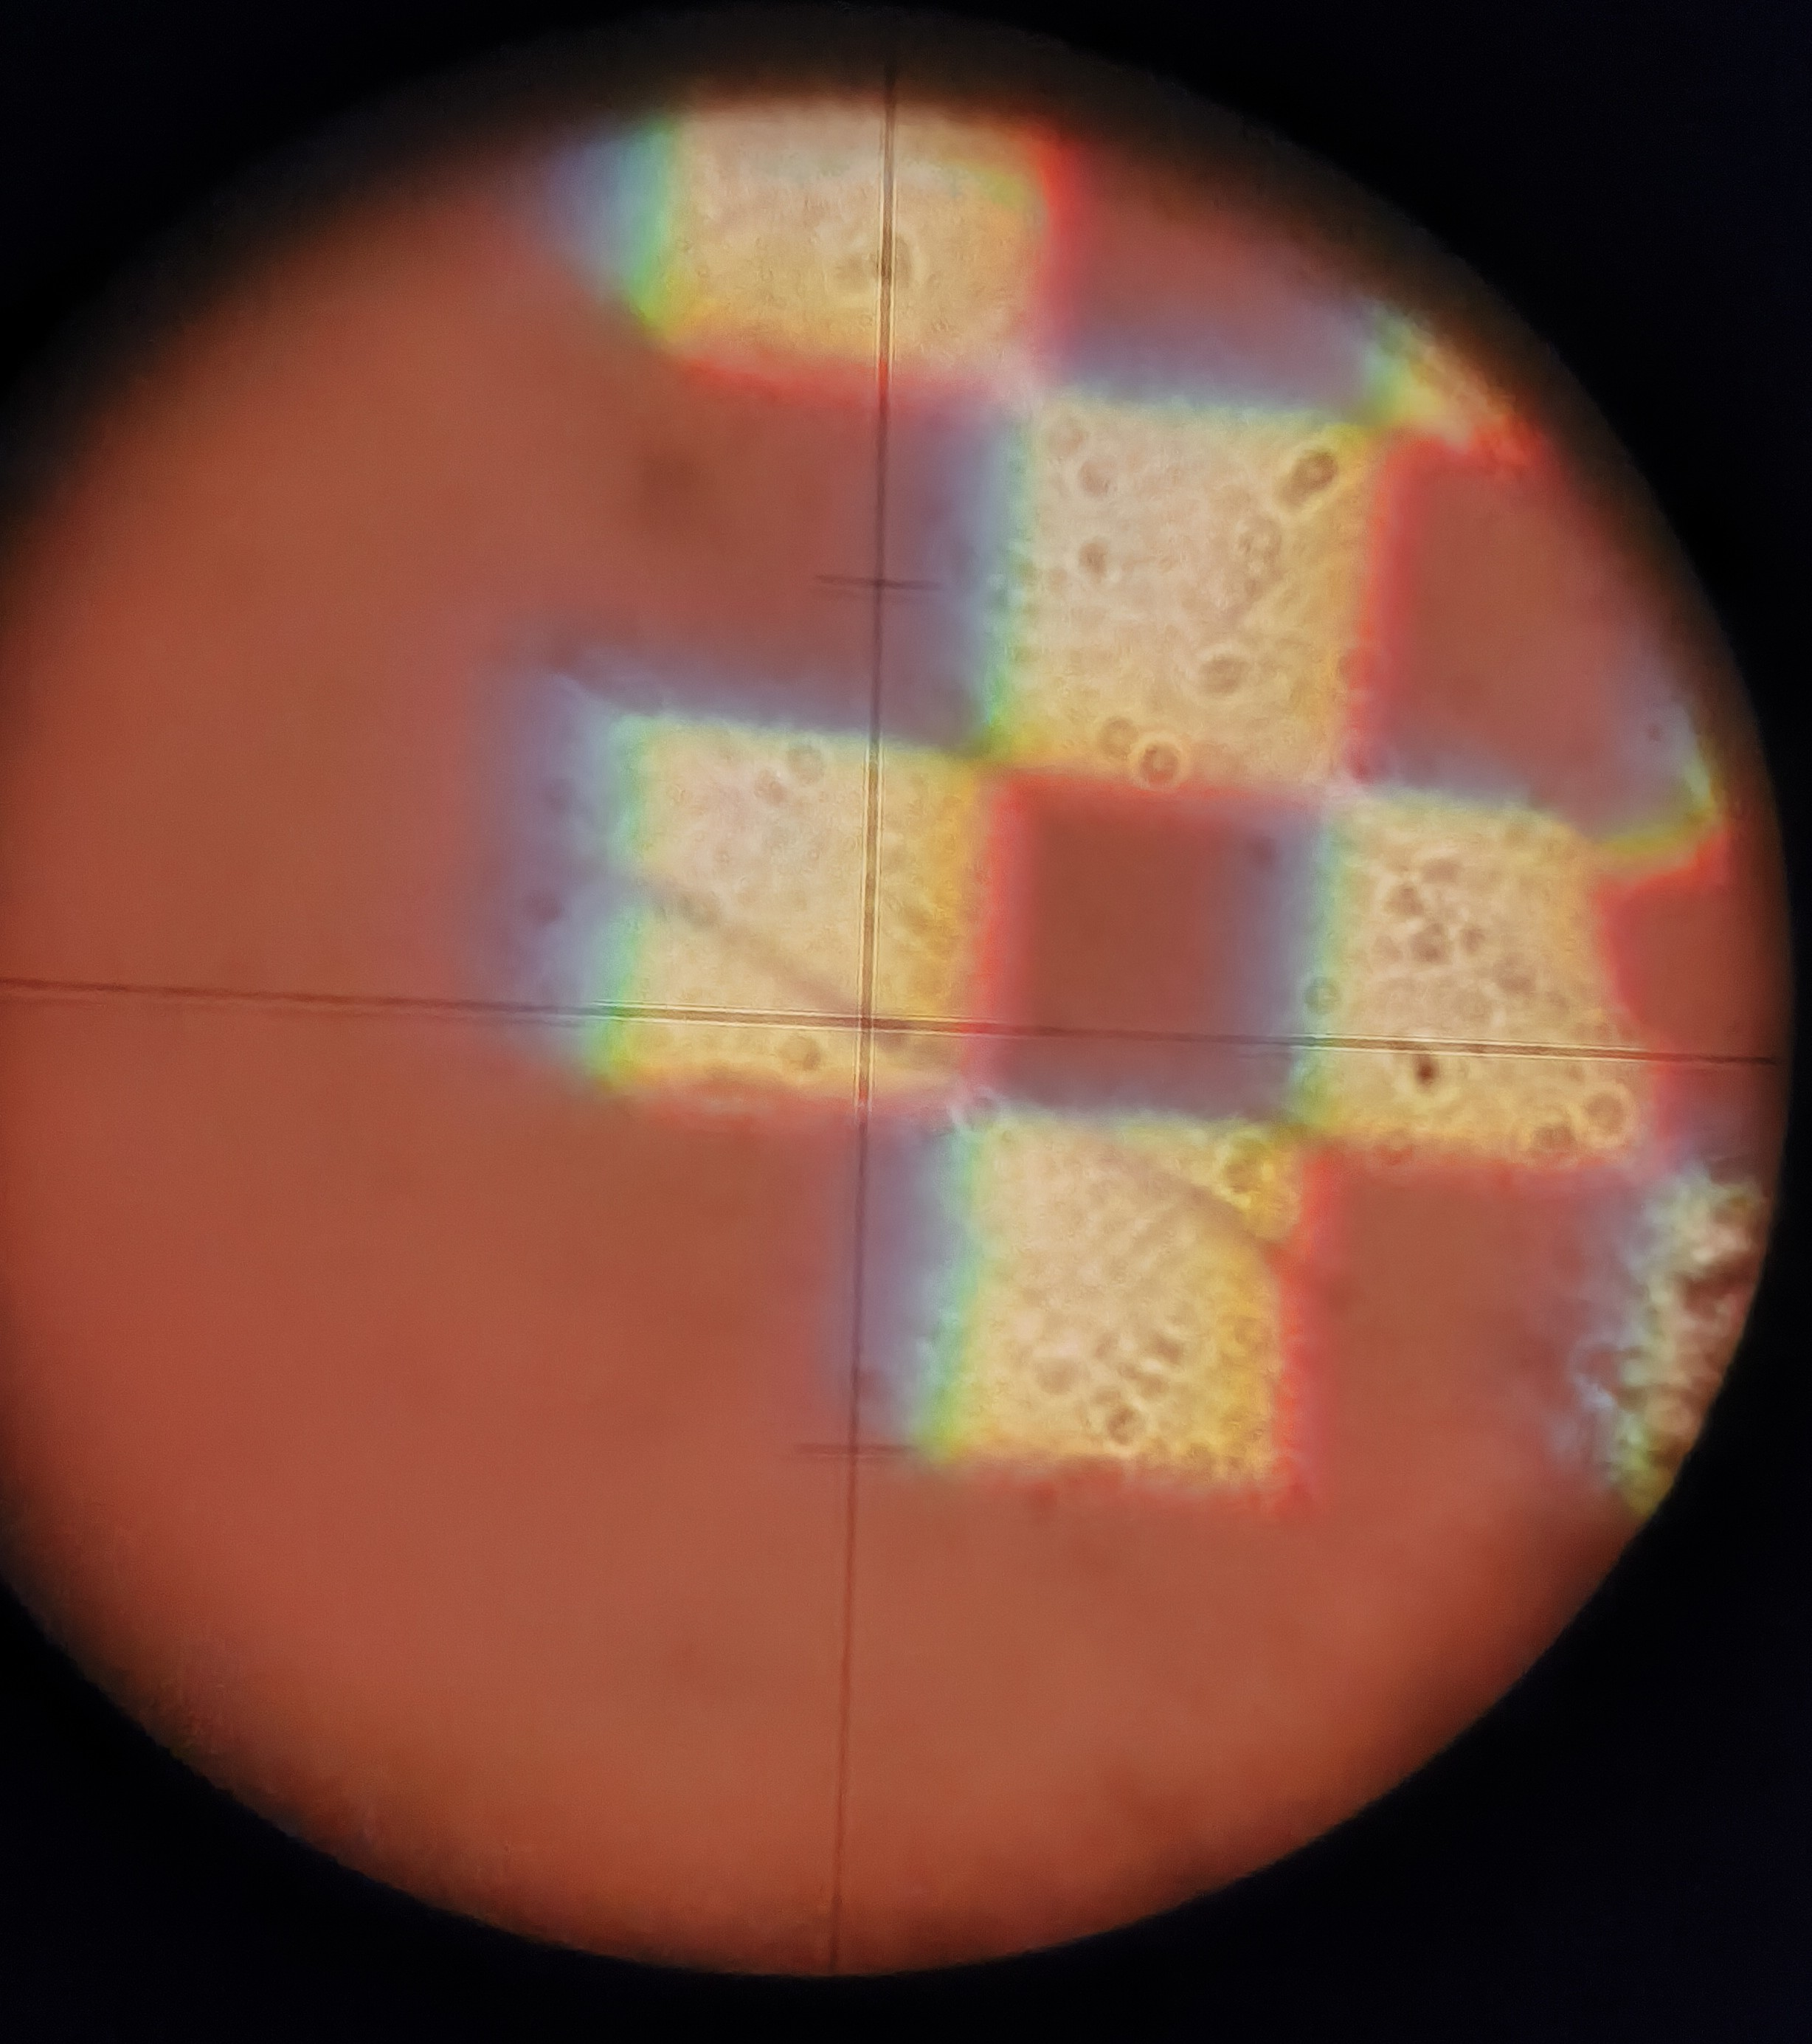
\includegraphics[width=0.4\linewidth]{f1.jpg}
	\label{pic_1}
\end{figure}

\section{Вывод}

Измерил фокусные расстояния линз разными способами. Собрал подзорную трубу Галлилея и подсчитал ее увеличение.

\end{document}